\chapter{Text Recognition Algorithms}

The root of any complex OCR software is text recognition. It is based on transforming an input image into its segmented form, with segments containing information about individual characters and their positions. In this chapter, we will analyze the individual steps that this process requires, along with a few obstacles the text recognition algorithms come across. These contribute to a poor quality of the given image and greatly impact the overall results. This leads to the conclusion that the software should behave according to them and try to solve these problems.

Firstly, we will therefore present the most common problems that lead to low image quality.

Secondly, we will demonstrate ways to solve them, which include image manipulation and the techniques of preprocessing. These try to minimize negative effects of poor quality images on text recognition algorithms.

Only once the preprocessing part is done can we move onto the actual recognition. This also consists of multiple steps. To detect characters or symbols in an image, we firstly need to segment the image into simpler parts that are easier to recognize. The individual techniques and types of segmentation, along with data representation are also thoroughly analyzed in this chapter. The last step of the algorithm discussed is actual character recognition from small segments and their transformation into a text format.

In this chapter, we also present an overview of some of the most popular optical character recognition software, including Tesseract, that is used in our implementation.

\section{Text Recognition Problems}

\xxx{meno tejto sekcie ok?}

Text recognition algorithms are most likely deemed to fail when the image presented is of low quality. This is because, similarly to the human eye, the software expects a significant difference between the characters and the background, expects parts of the images that represent the same character to look the same and is accustomed to working with aligned and properly straightened images.

In their paper, \citet{preprocessAll} describe the following major difficulties that complicate the text recognition process:

\begin{description}
\item[Font face variability] Nowadays, a multitude of different fonts and styles is used in the documents. This includes different headers and footers, headings and body text, along with bold, italics and underlined characters, not to even mention differently colored fonts and even custom-made fonts. To hold the information about each and every one would be unsustainable for any OCR software, and, in case of custom-made fonts, even impossible, as there is currently no database of all existing fonts. Therefore, the OCR software needs to make assumptions and use heuristics to match its expectation of the character shape with the actual symbol it recognized.
\item[Handwritten text] Handwritten text is usually perceived as a type of more complicated font. On contrary to typical machine fonts, the characters that are supposed to be the same do not always have to look that way. This is why the OCR software has to count on minor character mistakes. These depend on different factors, such as line height, length, character size and others. Furthermore, handwriting can sometimes be unrecognizable even by a human eye. This case often prompts the software to fail.
\item[Scan quality] Poor scanning process or just poor initial image may cause suboptimal performance of the recognition algorithm. The image can be low-contrasted, not sharp enough, lines can be disrupted or pixelated (mostly in case of a low scan resolution), or it can contain a lot of noise. These problems are usually partly solved during the preprocessing part of OCR algorithm.
\item[Skew problems] Images that are skewed also come under the part of preprocessing. As the result of a scan or even a photography is almost never an image with a perfectly aligned text as it was on the paper, this needs to fixed, so the actual algorithm can count on correctly aligned images.
\item[Colors] As already mentioned before, OCR softwares work on the basis of distinguishing characters from the background. This leads to a simple observation --- the better the contrast of the image, the better the OCR results. Colored images generally have a lower contrast than when they are in black and white. Furthermore, there is no need for OCR software to keep the color information during the process, as it would only significantly complicate detection and increase time. Before passing to OCR, images therefore undergo binarization.
\item[Glyph similarity] Even people sometimes make mistakes when distinguishing characters like S and 5, O and 0, or I and l. OCR software can often make the same mistake, especially when handling documents that use various numbers of fonts \xxx{toto je ok?}, decorative fonts, or even  handwritten text.
\end{description}

These and multiple other factors are also the reason why the majority of OCR software works with `assumptions' about documents --- that the document has only one column, is not handwritten, that its lines are horizontally aligned and so on. Also, this is why no OCR software can work perfectly and will always keep encountering documents that are unrecoverable. 

However, there are many ways in which we can improve the results of the OCR. They either try to solve the already mentioned problems by processes like deskewing, image enhancement, denoising, or they simply increase the performance of OCR engines, like binarization. We will cover them thoroughly in the next section.

\section{Preprocessing}

Many of the existing OCR engines already come with some kind of built-in preprocessing filter. Their problem is that they most likely do not match the exact image case and are usually very simple.

This is why the best practice is to firstly preprocess the image and then pass the result to the OCR algorithm.

In this section, we will discuss the most important image transformation that we can perform to improve the results of the OCR. 

\subsection{Scaling}

\xxx{tak celkovo neviem co s touto sekciou. Pride mi zbytocne obrovska na to, ze tuto moznost vobec ani v bakalarke nemam, ale kedze som to pisala samozrejme mi je luto z tade hocico vyhodit :D}

OCR usually benefits from a properly scaled image with good resolution. It contains more detailed information that can be used to interpret text, which leads to higher accuracy of the result. This can be specifically applied to the case of resolution and bit-depth.

Many popular OCR engines (e.g. Tesseract \citep{TesseractQual}, ABBYY FineReader \citep{ABBYYdpi}) encourage their users to use 300dpi images. Their reason for that is pretty simple - it is the point where they gain the most accuracy without sacrificing speed and file size. After running a few tests for the same image with different resolution on OCR engines \citep{preprocessAll}, the improvement gap between 200dpi scan and 300dpi scan is at least 2 times the improvement gap of any other resolutions. Also, when comparing other images above 300dpi with a 300dpi image, the improvement gap is nearly absent. It is obviously still there, but in almost all cases, the higher resolution is not worth the time and space. 

Another reason for the use of 300dpi is the fact that most OCR engines are trained to this resolution. Some engines (like the already mentioned ABBYY FineReader \citep{ABBYYdpi}), no matter what resolution you give them will actually sample up or down to get to 300dpi. 

Obtaining a 300dpi scan using currently available hardware is simple enough. If the user has already provided us with an image of a different resolution, our next steps depend on what the resolution is.

\begin{description}
\item[Lower-resolution images] \todo{tohle je na description moc dlouhy, asi chces subsections. Mozna pojmenovany jako `upscaling' a `downscaling'.} Simply scaling the image would leave the result pixelated, blurred and not sharp enough. The most affected parts would be the diagonal edges of elements. They would appear jagged (\emph{aliased}), which gives the image overall a poor quality. To minimize this unwanted effect, a technique called \emph{interpolation} is used.

Interpolation works by using known data to estimate values at unknown points. It specifically approximates the resulting pixel's color and intensity based on the values at surrounding pixels. It therefore already includes the process of \emph{anti-aliasing} (process used to minimize aliases), as it is based on the same technique.

The more data we have, the better the interpolation - therefore we will still see the difference between a resized image from 72dpi to 300dpi and 200dpi to 300dpi.

Interpolation algorithms can be grouped into two categories: \emph{adaptive} and \emph{non-adaptive}. Non-adaptive methods treat all pixels equally, while adaptive methods change depending on what they are interpolating, specifically smooth texture vs. sharp edges. Adaptive methods are primarily designed to minimize the presence of interpolation artifacts in regions where they are most apparent, and they differ by the way they detect edges.

Non-adaptive methods do not distinct \todo{distinguish? make a distinction between?} different pixels. Their complexity depends on the number of adjacent pixels during interpolation, which is also the criterion by which the existing methods are classified~\cite{interpolation}. \todo{doplnil jsem uvod seznamu} The usual non-adaptive methods include:

\begin{itemize}
\item \emph{Nearest Neighbor Interpolation}\todo{Odstranil jsem bold --- bold je navigace. Kdyz chces definovat nejaky terminy nebo nazvy, emph je nejlepsi volba.}, which uses only the value from the pixel that is closest to the interpolated point.

\item \emph{Bilinear Interpolation}, which considers the closest $2\times2$ \todo{of pixels? milimeters? glyphs?} neighborhood of known pixel values surrounding the unknown pixel. It then assigns the weighted average of these 4 pixels to the final interpolated value.

\item \emph{Bicubic Interpolation}, that \xxx{goes one step}\todo{does it literally walk? Asi chces rict improves?} beyond bilinear and takes the closest \xxx{4x4} neighbours, which sums up to the total of 16 pixels. During the calculation of the final value, pixels closer to the interpolated point are given a higher weighting.
\end{itemize}

There also exist higher order interpolations, such as \emph{Spline}, \emph{Sinc}, \emph{Lanczos} or \emph{Discrete Wavelet Transforms}~\cite{interpolation}. These consider more surrounding pixels and calculate the resulting value through more complex functions, like transforms or sampling functions. The results are more accurate than those of simple calculations at the cost of significantly more time. For the purposes of OCR, such complex and time-consuming functions are not desirable, as we are not yet working with any rotations and distortions and just need to resize the existing image.

For the best quality/time ratio, the popular decision in most cases is \emph{Bicubic Interpolation}. Although \emph{Neareast Neighbor} and \emph{Bilinear} methods are extremely fast, the results were found to be poor~\cite{interpolationComp}.

\item[High-resolution images] In case the user supplies an image with resolution higher than 300dpi, we need to solve the exact opposite problem as previously - decrease the number of pixels and decide what will the values of the new ones be. The easiest approach would be to "pick every nth pixel", but the same problems as previously arise - blurring, aliasing, pixelation\ldots

The simplest and most widely used approaches are very similar to what is already explained above. To calculate the value of the resulting pixel, we choose a number of surrounding pixels. We calculate their weighted average and assign this value to the unknown pixel. As previously, the 4x4 neighborhood turned out to have the best quality/time ratio.

There are obviously many other ways that our desired result can be achieved. Already mentioned \emph{Spline}, \emph{Sinc}, \emph{Lanczos} and other "reverse interpolations" are a few of them. Worth noting are also \emph{Fourier transformation}, \emph{perceptual based methods}, \emph{content-adaptive methods} and other adaptive and heuristic techniques.
Many of these methods produce even better results, but, as mentioned before, most preprocessing engines still stick to the simpler "reversed Bicubic Interpolation" in a successful attempt to speed up the algorithm.

\end{description}

\subsection{Contrast enhancement}

Another important factor that results in low-quality images is low contrast. Even human eye has a harder time recognizing images 
with this element, and the same goes for OCR engines. 

An image \emph{histogram} is used to improve this aspect. It is an accurate representation of the distribution of data and, in case of image histograms, it represents the tonal distribution of an image - x-asis in histogram stands for all available tonal levels, and y-axis represents the number of pixels for each tonal level.

Grayscale images are represented by only one histogram, where the x-axis contains all the available grey values. However, in colored (RGB) images, the histogram is displayed by the terms of three separate histograms\xxx{ - }one for each color component (R, G and B). Increasing contrast for colored pictures is therefore a more complex task. This, however, is not a case we need to solve, as the next part of preprocessing is binarization. As we will mention later, binarization works better on grayscale images. Therefore, the conversion to grayscale can already be performed in this section. Only after that, the contrast enhancement will take place.

\textbf{Grayscale conversion} \todo{tohle asi zas muze byt subsection} is the process of computing and assigning the grey value for each colored pixel from its attributes. There exist a few different approaches to this problem, \xxx{with the most simple one being}\todo{mozna chces oddelit vetu ve ktery reknes ze napr. averaging je nejjednodussi, protoze proste jen prumeruje RGB.} the averaging approach. This method assigns each pixel the average of its R, G and B value. However, this does not really preserve the brightness of the image\todo{it preserves the brightness defined from average! :D}. For that reason, advanced correction based on the perception of human eye (often called \emph{luma}~\cite{grayscaleConv}) is used. This algorithm \todo{is that really an algoritm? Mozna: `formula', `method', `conversion'} \xxx{takes notice of}\todo{exploits? reflects?} the fact that human perception of different colors is non-uniform (green \todo{green part of the spectrum?} is perceived more strongly than red, and red more strongly than blue). Because of this, each color component is weighted in the resulting formula. Another way to approach grayscale converstion is to represents the color based on its HSL values and convert it to its least saturated variant.

As decribed by~\citet{grayscaleCadik}, these exist many more algorithms approaching this problem. Most of them require more complicated computations and try to preserve attributes of the image that may be lost during the process --- like contrast or luminance.

Now that we have a grayscale image\todo{but we didn't produce any. Mozna: After obtaining a suitable greyscale image?}, the next step is contrast enhancement \todo{the next step is....the processing usually continues with?} with the help of already mentioned histograms. \xxx{In them, contrast} is represented as distribution of pixels\todo{pixel luminance values?}. The more evenly the pixel counts cover a broad range of grayscale levels, the better the contrast of the image\todo{to neni uplne pravda, nejkontrastnejsi obrazky maj uprostred histogramu diru, coz neni uplne `evenly'.}. Pixel counts that are restricted to a smaller range indicate low contrast\todo{ve skutecnosti to je low luminance range}.

To obtain an image with higher contrast, we therefore need to \xxx{stretch its histogram}\todo{kdyz vemes uplne celej histogram a roztahnes ho, tak se ve skutecnosti nic nezmeni}. In the following \xxx{paragraph}, we will briefly explain the basis of a few of the most popular methods. However, many more complex and complicated techniques already exist, including CLAHE\todo{citace na tohle je v ty spolecny?}, Dynamic Stochastic Resonance and generic transforms, such as Fourier, Discrete Cosine, and Wavelet~\cite{contrastOther}.\todo{Odpalil jsem hodne emph --- je to potreba jen kdyz definujes nejakej pojem kterej si clovek ma precist 10x a nutne zapamatovat protoze o nem budes jeste mluvit; tim ze emphasisem oznacis vsechno nutis ctenare pokusit se zapamatovat si moc veci najednou a nasledne v tom mit chaos.}

\begin{itemize}

\item The \emph{linear stretching} method linearly expands the original digital values of the histogram into a new distribution. There exist three methods of linear stretching - \emph{Min-Max}, \emph{Percentage} and \emph{Piecewise} Contrast Stretch \citet{linearNonStretch}. All these methods make subtle variations within the image data more obvious, are are best applied to remotely sensed images with Gaussian or near-Gaussian histograms.

\item\emph{Non-linear stretching} is done by functions with non-linear form. These include logarithmic transform, exponential transform or Power Law~\citep{linearNonStretch}. The downside of these methods is that each value in the input image can have several values in the output image - therefore, the objects in the original scene lose their correct relative brightness value.

\item\emph{Histogram equalization} is one of the most popular methods based off non-linear stretching. It is based on transforms that depend on the probability distribution function of the histogram~\citep{histogramEQ}. Although it produces unrealistic effects in photographs, it is widely used for scientific images.

\end{itemize}

For text image enhancement, the most popular choice is histogram equalization, or, in more complex cases, CLAHE. However, as always, different images require different processing techniques.

\subsection{Binarization}

As already mentioned, element detection in color, or even greyscale images is a way more complicated task than with monochrome one (1 bit) images. This is due to the the lack of contrast and therefore possible blending of different edges during recognition.

Binarization is a process that converts an image to its monochrome one form. This means that every pixel on the binarized image will be either black or white.

Many binarization algorithms work under the assumption that the input image is already in greyscale. If not, they firstly transform the image to greyscale, then apply the binarization techniques. This does not concern us, though. In the last section, where we talked about contrast enhancement of the image, our results were already in greyscale. Therefore, for the next part, let us assume that the images we work with are strictly in greyscale.

The simplest approach to binarization is \emph{global thresholding} \citep{globalThresh}. It works by choosing a threshold value and iterating over the whole image, comparing the value of each pixel to this threshold. If it is greater, the pixel in resulting image will be black, otherwise white. As the brightness and contrast of different images vary, it is impossible to choose a threshold suitable for all images.

Therefore, other more complex methods are used:

\begin{itemize}
\item\textbf{Otsu's method} \citep{otsu} is one of the most widely used and mentioned methods for image binarization. First, it computes the threshold value from the input image and then applies global thresholding. To get the optimal value of the threshold, Otsu's method works by dividing the pixels into two groups - background and foreground pixels. It chooses these groups so that the within-group variance is minimized and between-group variance is maximized. Upside to this method is that it is simple and easy to implement. However, upon applying it to images with uneven dark or bright spots, it deems to be unusable.

\item\textbf{Local Thresholding} \citep{localOtherBin} differs from Otsu's method by assigning different threshold values to the segments of the image. This solves the problem with unevenly lit spots --- darker spots will be assigned a lower threshold value, while brighter will be assigned a higher threshold value. The difference between different local thresholding algorithms is the way the values are assigned. For example, \emph{Niblack's Method} \citep{adaptiveBin} determines the threshold of every pixel by using the mean and standard deviation of surrounding pixels, which causes errors in blank regions of the image. \emph{Sauvola Method} \citep{adaptiveBin} improves this by using the dynamic range of image gray-value standard deviation. However, this often results in text thinning. Another method worth mentioning is \emph{Bernsen's} \citep{adaptiveBin}, where the threshold is set to the mean value between the lowest and highest gray-level pixel in the neighborhood.

\item\textbf{Adaptive methods} attempt to overcome the fact that every document is different and techniques that work for a few inputs may substantially corrupt others. To determine which technique to use for each document image would be a useful feature in most cases. This is the exact problem that adaptive methods try to solve. As described in \citep{adaptiveBin}, their approach is to analyze the document image surface and determine the most useful method with the help of a "hybrid switching" module.

\end{itemize}

Comprehensive reviews of other, more complicated methods (mostly based on already mentioned techniques) are available \citet{localOtherBin}.

\subsection{Deskewing}

Skewed images are probably the most common problem that many OCR engines struggle with. They usually appear when an image is scanned or photographed crookedly. 

One of the steps of OCR algorithms is \emph{page segmentation}. It is the process that decomposes a document image into elements. This division is based on vertically and horizontally aligned characters, spaces and other elements. If the documents have Manhattan layout, decomposition is even easier and can be done by vertical and horizontal cuts. We will discuss this topic thoroughly in the following chapter. For now, the important thing to know is that skewed images pass misaligned data to the OCR algorithm. This causes more errors and ultimately leads to poorer results.

There are different approaches that deal with this problem. All of these methods work (for more accurate results) after binarization of the image and generally assume the skew angle to be no more than 15$^{\circ}$. Algorithms that work on greater skew angles also exist\citep{skewAngleDetection}. They are not as widely used, though, as most of the time, correction needs to be done on scanned documents - which are mostly only slightly tweaked.

As described by \citet{skewBestTechniques}, the most effective deskewing algorithms include the following:

\begin{itemize}

\item\textbf{Hough Transform:} This method is used to find straight lines in an image and given their rotation, determine the skew angle of the whole documents. It is based on a feature extraction technique called \emph{Hough Transform} \citep{houghTransform}. This method is applied on different lines. Then, it determines which line is the most represented in the input image by comparing their number of pixels. Only thing left is the computation of the resulting angle. Although highly effective, computations of transform can be quite time consuming. This is why the transform is usually not done on every point of the image, but only a set of chosen input points. Another problem occurs if pictures or other graphic data are present in the input image (as Hough Transform counts with aligned pixels). To solve this, we only choose input points from the text data.

\item\textbf{Projection Profile: } Projection Profile method is based on creating a histogram of black pixels along horizontal or vertical scan lines. For an image with horizontal scan lines, this histogram will have peaks at text line positions. The algorithm estimates the skew by rotating the image in different angles and comparing the resulting histograms. The one with the most peaks and valleys belongs to our final angle. The problem with this technique is that it works on text areas only, as images or other elements can disrupt the histograms.

\item\textbf{Cross Corelation} works similarly to Projection Profile method mentioned above. Firstly, it selects a number of vertical segments from the image. It then performs the Projection Profile algorithm on these segments and by comparing then, it can estimate the final skew angle. The drawbacks of this method are similar to those of Projection Profile. However, it usually needs to process less data with no loss in accuracy, given a good choice for the width of the columns.

\item\textbf{Connected Component Clustering} - or \emph{Nearest Neighbor Clustering}. Thoroughly described in \citet{skewClustering}, these algorithms are based on finding coherency between connected components of the image. They either compute the skew of every component (using their bottom line) and compare the results, or group components by neighbours and create a group histogram for examination or many other more.

\end{itemize}

Worth noting are also other methods like \emph{Fourier} \citep{fourierTransform}, \emph{Wavelet Decomposition}, \emph{Radon Transform}, \emph{PCP}, \emph{one-pass} or \emph{multi-pass} skew correction, \emph{morphology algorithms}\ldots \citep{skewBestTechniques}.

\subsection{Noise reduction}

Image noise is an usually unwanted random variation of brightness or color information in images, reminding film grain in digital cameras. It is often caused by the sensor of a scanner or a digital camera attempting to record small amounts of light. 

For OCR engines, processing noise can be quite tricky. Its presence is especially crucial during binarization and edge detection. These processes are based on the differences between the "outside" of the element and its "inside". When noise is present, it can disrupt these borders, which can often cause the failure of recognition.

Based on the way they originate and are processed, we concentrate on these types of noise:

\begin{itemize}
\item\textbf{salt and pepper noise}, also known as \emph{impulse noise}, can be recognized as randomly occurring black and white pixels. It is caused by sharp and sudden disturbances in the image signal, and can be most likely seen on old photographs.

\item\textbf{statistical noise\xxx{ - }} is an unexplained variability within an image. It is characterized by a probability density function. Most common is \emph{Gaussian noise}, \emph{Shot noise}, \emph{Quantization noise} or film grain.

\item\textbf{other} - like \emph{anisotropic} or \emph{periodic} noise. These are often found on old photographs or documents.

\end{itemize}

There exist various approaches dealing with noise reduction. These include different types of filtering or comparison methods to firstly detect which pixels were corrupted by noise and then determining their value in the output image.

\begin{description}

\item One of the most commonly used techniques, found also in image editing software like Adobe Photoshop or GIMP, are \textbf{linear filters} \citep{denoisingTechniques}, like \emph{mean filter}, \emph{Gaussian filter} or \emph{Wiener filter}. They work on averaging the color values of neighbour pixels, so they can help assure an averaged view of the contrast along regions of different color. This, however, rather than correcting the color of the affected pixel, results in creating an area with an average (and incorrect) color. This blurs the edges and smooths out other fine details. They are still widely used, though, as they require only a small amount of computations, which leads to increased speed and easy and simple implementations.

\item Other filters used for image denoising include \textbf{non-linear filters} \citep{denoisingTechniques}. The most popular of them is \emph{median filter}. It works similarly like a mean filter, but for each pixel, instead of replacing its value with a mean of surrounding pixels, it calculates the median. In comparison with linear filters, it provides considerably sharper images and in cases preserves the edges. The downside is the increased run time, and with high level of noise, results are almost the same as with linear filters. However, it is highly effective on salt and pepper noise.

\item Worth mentioning is also \textbf{non-local means method} \citep{nonLocalMeans}. It is based on taking a mean value of all pixels of the image, weighted by how similar these pixels are to the target pixel. This technique produces an even sharper and clearer image results as mentioned filters. However, it comes with the expense of additional increased speed.

\end{description}

What combination of techniques to use for the optimal results greatly depends on the input image - if there is little to no noise, de-noising an image can cause more harm than good. Therefore, it is always important to approximately compute the signal:noise ratio before applying any kind of filters.

To calculate this properly is a more complex task than thought. Although simple algorithms have already existed for a few years, they return poor results and most of them are almost not worth using because of the time complexity. They are mostly based on comparison - testing the difference between each pixel and its neighbors for various threshold numbers based on the dynamic range and calculating deviation, picking "windows" of different sizes and calculating their means and deviation, based on which we decide whether the center pixel is corrupted or not and so on\ldots

For a more complex (and sufficient) solution, we have to run many more mathematical calculations on the input image \citep{noiseDetection}. These calculations require a lot of knowledge in the field of probability and statistics, specifically probability distribution. The basic idea for these noise recognition algorithms is \emph{separating frequencies}. This is usually done by dividing the image into blocks and running a transformation (for example a \emph{discrete cosine transformation}) on each of the blocks. The frequency components are then grouped by increasing frequency. Then, the extraction of statistical features (such as kurtosis, mean, standard deviation) is performed.

Noise is most likely to be found on higher frequencies and we use this observation along with our computed statistical features to determine the thresholding on higher frequencies. If the threshold of the input image is greater, the image is determined to be noise-free. 

\subsection{Scanning border reduction}

Scanned documents often have visible dark borders (\emph{marginal noise}). These are created either during scanning (due to the presence of neighbouring pages) or are an unwanted result of the binarization process.

Similarly to noise reduction, running this step could only be harmful if there is no marginal noise present. Therefore, the algorithm has to have two steps - \emph{marginal noise detection} and, if successful, \emph{marginal noise reduction}.

Marginal noise is present as a dark connected component of the page. This is a fact that most detection algorithms take advantage of. Firstly, they extract the connected components of the page. This can be done by a \emph{black filter} (a moving rectangular window that calculates the ratio of black pixels on border \citep{marginalNoiseWindow}). After obtaining the connected components, different heuristics are used - most based on removing the connected components near the edges. In the end, usually a "cleanup" is performed (like \emph{white filter} \citep{marginalNoiseWindow}) - for removing all unnecessary elements around the borders (an unwanted text from the neighbour page, noisy components in the corners\ldots).
The results of this algorithm depend greatly on the values of thresholds, margings and other hardcoded parameters. Different images work well under different values. This is why the cleanup part's parameters are usually dependant of the results of previous parts.

Another approach is the one mentioned by \citet{marginalNoiseEdge}. It is based on edge density calculations, and the fact that text areas have generally a much lower density than edge areas. An edge detector (in this case, \emph{sobel}) is used for examining vertical marginal noise, and later horizontal marginal noise. It returns the positions of the margins. Anything beyond these positions is detected as an unwanted noise, and can be therefore removed by filters or other removal algorithms.

\section{Text detection process}

Nowadays, two approaches are proposed for text detection in OCR. The first one is an approach based on heuristics --- page segmentation, line and element detection and only after that, character detection, which is based on different approximations and sometimes naive algorithms. The second one is an approach that is widely used and researched today --- and that is the use of neural networks.

In this paper, we will be concentrating on the heuristics approach of the OCR problem, as we use it in our implementation. However, neural network recognition is nowadays an approach returning \xxx{?? spravne?} promising results and also deserves a mention.

A lot of OCR engines differ in the way their heuristic approaches work. They all agree on one thing, though, and that is the succession of steps that need to be implemented. Firstly, a \emph{page segmentation} has to be performed. This divides the given page into multiple segments that are easier to process when determining the elements of the image. Now, the recognition algorithm could simply take place. However, most of the existing OCR engines (like Tesseract) "pre-process" the output of page segmentation. They use steps like \emph{representation} and \emph{feature extraction}, which are based on simplifying the extracted elements of image documents. This contributes to better results of the OCR, and, last but not least, helps to improve the speed of the algorithm.

Only after this, the character recognition algorithm is applied.

We will analyze these steps in the following individual subsections.

\subsection{Page Segmentation}

In many cases, OCR system heavily depends on the accuracy of page segmentation process \citep{pageSegmentation}. There are three main approaches \citep{segmentationBenchmark} to this problem --- either we start with an image as a whole and recursively divide it into parts until criterion is met, or we start with individual pixels and group them according to similarity of their attributes, or we use a combination of these two methods. Based on these methods, there exist a few concrete algorithms widely used for heuristic page segmentation.

\subsubsection{Page Segmentation Techniques}

\xxx{TO DO - chcem dat captions tym fboxom, netusim vobec ako}

\clearpage

\begin{longtable}{p{7em}p{13em}c}
\toprule
\textbf{Page} & \textbf{Description} & \textbf{Image} \\
\textbf{Segmentation} & & \\
\textbf{Algorithm} & & \\
\midrule
RXYC

algorithm

(\emph{X-Y cut})
&

one of the oldest and simplest methods

tree based algorithm, works by recursively splitting the nodes of the tree into rectangular parts

uses projection profile and threshold computations for determination of splitting

easy to implement, fast

usually fails at the presence of imperfections

&
\fbox{\raisebox{-\height}{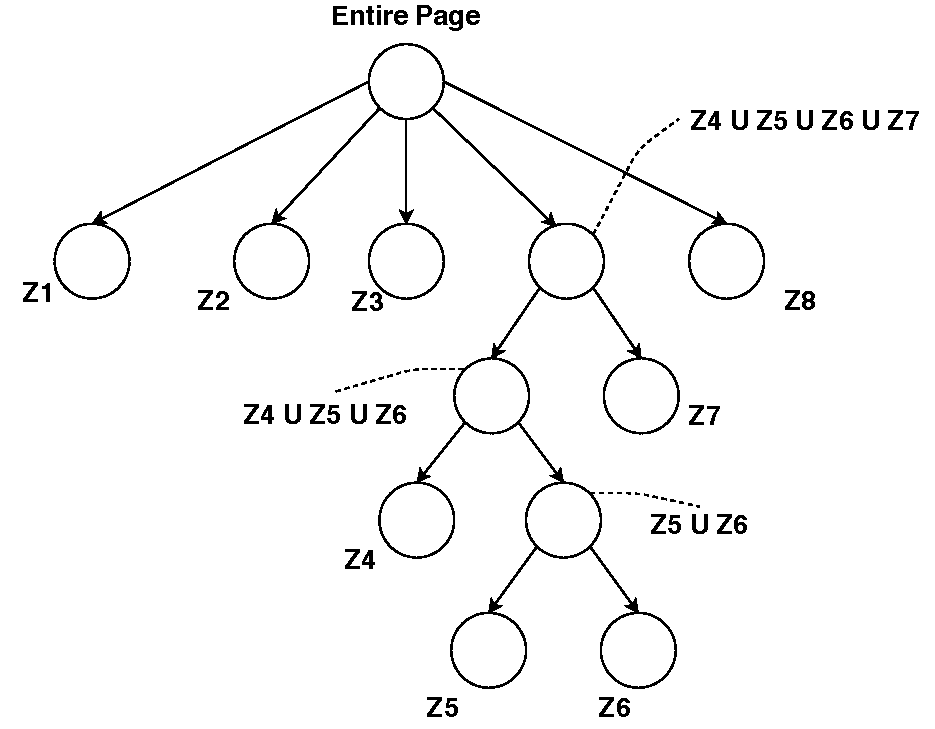
\includegraphics[width=0.3\textwidth,
height=40mm]{img/segm_rxyc.pdf}}}\\
Smearing 

algorithm 

(\emph{RLSA})
&

based on linking together black areas that are no more than C pixels away from each other

requires binarized images

slightly better results than \emph{X-Y cut}

fails at the presence of noise, not used for text documents

widely popular among vehicle plate recognition
 &
\fbox{\raisebox{-\height}{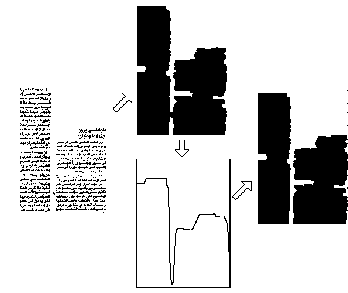
\includegraphics[width=0.3\textwidth,
height=40mm]{img/segm_smearing.png}}}\\
Voronoi

diagram 

based

algorithm&

bottom-up algorithm

performs a noise removal 

creates Voronoi diagram from sample points of edges of extracted connected components of the existing image

performs a "clean-up" of the diagram - deletion of superfluous edges

can be used on documents with noise and other imperfections

causing over-segmentation errors when working with documents using different fonts or styles

advised to use on homogeneous collection of documents &
\fbox{\raisebox{-\height}{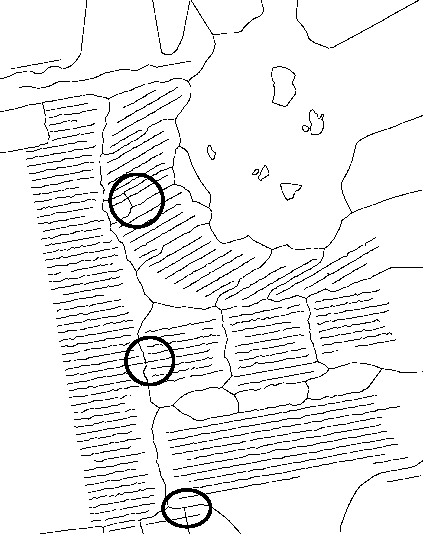
\includegraphics[width=0.3\textwidth,
height=60mm]{img/segm_voronoi.png}}}\\
Docstrum

algorithm

&

bottom-up algorithm

based on fonts and styles of the characters

divides connected components into a dominant font group and a group with characters from titles or sections heading

performs a near-neighor clustering of components in each group

determines the skew of the image and text-lines, upon which merges within-line nearest neighbor pairs into text-lines and blocks

similar errors like \emph{Voronoi diagram} algorithm

advised to use on a homogeneous collection of documents
&
\fbox{
\raisebox{-\height}{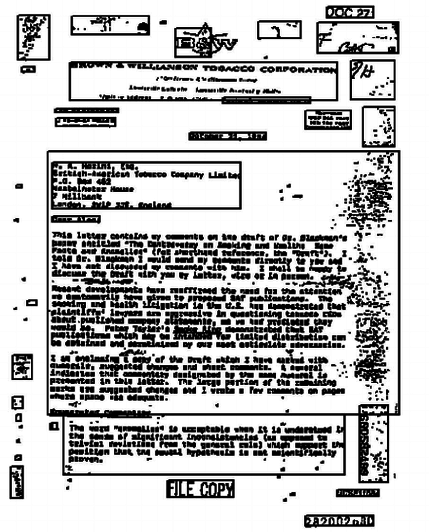
\includegraphics[width=0.3\textwidth,
height=60mm]{img/segm_docstrum.png}}}\\
Whitespace

analysis

&

assumes a white background of the image

finds a union of white rectangles as a cover of the background

uncovered regions of the image after applying the union are the results of segmentation

satisfactory results on heterogeneous documents

tends to result in either over-segmentation or under-segmentation depending on the sizes of rectangles in the union

overall, performs worse than \emph{Voronoi} or \emph{Docstrum} algorithm
&
\fbox{
\raisebox{-\height}{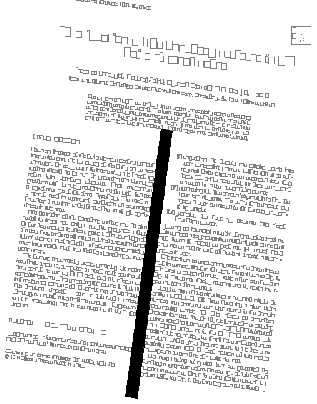
\includegraphics[width=0.3\textwidth,
height=60mm]{img/segm_whitespace.png}}}\\
Constrained

text-line

detection
&

similar to \emph{whitespace analysis}, differs in the approach of finding the whitespace rectangles that cover the page background

good option for documents with different font sizes or layouts

nearly parameter free
&
\fbox{
\raisebox{-\height}{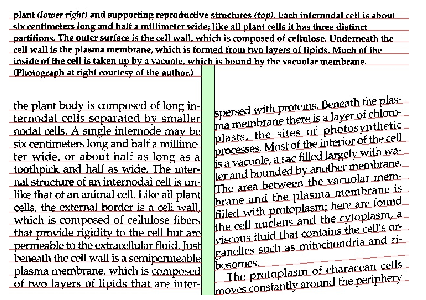
\includegraphics[width=0.3\textwidth,
height=60mm]{img/segm_textline.png}}}\\
\bottomrule
\caption{Page Segmentation Algorithms}
\label{tab:page_seg_algorithms}
\end{longtable}

\subsubsection{Tesseract page segmentation}

Another slightly different segmentation technique was proposed by \citet{tesseractSegmentationTab}. This method is based on detecting so-called \emph{tab-stops}.

\emph{Tab-stops} are used in word processors to enable correct and eye pleasing alignment of text, and are present in the document as margins, column edges, indentations. All of them are placed at fixed x-positions at which edges or centers of text lines are vertically aligned. This process has multiple steps. Firstly, it preprocesses the document image for connected components. By grouping these connected components into vertical lines and examining their vertical alignment, tab-lines are then detected, which mark the text-lines with their beginning and end. Based on these tab-lines, connected components of the page layout analysis are then grouped into \emph{column partitions}, which do not cross any tab-lines and are of the same type. In the end, a few of the column partitions can be merged or divided into segmented blocks, based on different types of fonts or line spacing. 

This method is implemented and used by the Tesseract engine, with the preprocessing help of the Leptonica library. It claims to yield satisfactory results, given the input document is properly preprocessed.

As our implementation uses the Tesseract engine for symbol recognition, this is also the method of page segmentation that it uses.

\begin{figure}
    \noindent
	\makebox[\textwidth]{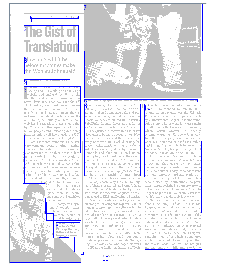
\includegraphics[width=20em]
	{../img/segm_tabstop.pdf}}
	\caption{Tesseract Engine Segmentation}
	\label{fig:mff}
\end{figure}

There exist many other segmentation methods that approach this problem differently. For example, with segmentation of scanned books that mostly have Manhattan layout, a simple deskewing and horizontal and vertical cuts should suffice. Also, algorithms focusing on recipe or ticket analysis already know what the approximate layout of the received image will be. They can therefore simplify these complicated algorithms for their purposes.

\subsection{Representation and feature extraction}

Upon extracting elements by page segmentation, we are left with an unnecessary amount of information. We could feed all of them into a recognizer. This would, however, decrease accuracy of recognition and significantly increase its time complexity. For these reasons, a set of features is extracted for each element that distinguishes it from other classes while keeping characteristic differences. This can be \xxx{done in various ways} \citep{featureExtractionBook}.

\todo{description list bez termu opet nejde pouzit, chces to predelat na tabulku nebo nejakej normalni seznam}
\begin{itemize}

\item The first group of techniques we will discuss are the \textbf{global transformation and series expansion} \todo{proc bold?}
\xxx{nejak som chcela dat nadpis tomu itemu a toto vyzera ze to tak zvyraznuje, mam dat emph?} methods. These include methods like Fourier or Gabor transform, Fourier Descriptor,Wavelets, Moments and Karhunen-Loeve expansion, and are based on the representation of continuous signals by a linear combination of simpler functions. The coefficients of the linear combination provide a compact encoding known as transformation or series expansion. Deformations like translation and rotations are invariant under global transformation and series expansion.

\item Another \todo{Je hlavni vlastnost statistickejch reprezentaci, ze jsou `another'?} representation and following extraction technique is \textbf{statistical representation}. Unlike transforms, it uses a statistical distribution of points to take care of font and style variations to some extend. Methods based on this representation are e.g. \emph{zoning}, \emph{crossings and distances} and \emph{projections}.\todo{Je to v necem lepsi nebo horsi nez ta prvni metoda?}

\item Various character can also be represented by their geometrical and topological features, based on the basic line types that form the character skeleton. The output of this representation and feature extraction process can be assigned into a feature vector.
This is called \textbf{geometrical and topological representation}, and includes techniques like \emph{extracting and counting topological structures}, \emph{measuring and approximating the geometrical properties}, \emph{coding} and \emph{graphs and trees}.\todo{tady ctenar absolutne nebude tusit co si pod tim predstavit --- jak se do toho vrazej ty grafy a stromy?}
\end{itemize}

\xxx{To sum up,}\todo{informal} the goal of any representation and feature extraction technique is to create a "skeleton" for each character by selecting the most representative information from the raw data which maximizes the recognition rate with the least amount of elements. However, these are still a number of differences between the features. The most noticeable difference is reconstructability - for some methods, the image can be reconstructed to its previous version solely because of features. Others, like statistical representation, lose information about the original image and would need complicated approximation algorithms to restore at least some of it. Another difference is the transformations to which features are invariant.

\subsection{Character classification}
\todo{Trosku problem je, ze na relativne jednoduchy metody pripravy textu spotrebujes 15 stranek a o hledani a klasifikaci pismen mas 1 sekci.}

OCR engines widely use the methodologies of pattern recognition, which assign an unknown sample into one of its predefined classes. There exist various approaches dealing with these methods, which are not necessarily independent of each other. Most often than not, OCR engines combine multiple methods to achieve the most accurate results.

One way to approach classification is by \emph{Template Matching} \citep{templateMatching}. It is based on the existence of predefined \emph{templates} --- multiple bitmaps containing characters of the alphabet. Improved version of this method have an extended database of templates, including numbers and special characters. Once a character is detected, it is passed to the algorithm and for every existing template, its similarity ratio is calculated. The template with the greatest ratio is then assumed to be the recognized character. This method has various implementation depending on how the ratio is calculated - for example \emph{cross correlation}, \emph{normalized correlation} or \emph{euclidean formula} can be used.

Although the implementation of this method is very simple, even small disfigurements and noise can greatly affect its efficiency. Also, in this case, a feature extraction would be unnecessary as all templates are created manually.

Another approach is by using \emph{statistical techniques}~\citep{characterClassification} that also make use of the previous steps mentioned in this thesis. They are based on statistical modeling of the data. To determine the output, extraction of the features from input image (such as size, shape, intensity) is first performed. Then, with the help of statistical decision functions, these features are compared to the statistical model.

The problem with these algorithms is that they have no information about whole-part relations. For this reason, a newer approach has been tested out over the past few years - \emph{machine learning} \citep{characterClassification}.

\emph{Machine Learning} \citet{sebastiani2002machine} is a method of data analysis based on artificial intelligence. Over time, it builds models of "training data". Based on them, it makes decisions and predictions on its input. 

In the case of character classification, training data is created by passing various characters into the engine and also providing it with the correct output. In this way, the engine learns how different characters should look and applies this knowledge to its input.

This method is for example used in a one of the simplest machine learning algorithms, and that is the \emph{KNN Classification Algorithm}, or K-Nearest Neighbor algorithm. The input image is compared to the training data and chooses its K nearest objects (objects that are the most similar). After that, the image is classified with being assigned to the class most common among its K nearest neighbors.

More complex methods include the \emph{Support Vector Machine algorithm} (SVM). This approach divides the data received into two classes - training and testing data. The goal of SVM technique is to deliver a model that predicts the output of the test set.

The learning is done by a \emph{SVM kernel}. The task of the kernel is to take the input data and transform it into the desired form using a combination of mathematical functions. Other than kernel functions, there are other parameters that tune the output of the SVM algorithm. \emph{Margin} parameter tells the engine the separation of line to the closest class points. \emph{Gamma} parameter decides how far the influence of a single training example reaches and \emph{regularization} parameter controls the misclassification of elements.

Many experiments have been executed in the field of machine learning for character classification. However, none of them can guarantee the accuracy of different approaches, as they all greatly depend on the training data. The more training data the machine can get, the more accurate it is. 

\section{Available OCR software}

\todo{Tahle kapitola ted nerika nic informativniho a do teoretickyho uvodu je uprimne dost zbytecna, myslim ze by bylo vhodnejsi ji presunout k implementaci (tam navic bude po ruce kdyz budes vysvetlovat proc to stavis na tesseractu) a nahradit nejakou vic comprehensive tabulkou ktera napr. nejak prehledne porovnava vlastnosti tech jednotlivych implementaci.}

\xxx{Over the past few years, OCR has become a part of our everyday lives.}\todo{nein} The demand for a reliable OCR engines has therefore risen, which lead to many new implementations or improvements of the already existing ones.

Most people take the expression "optical character recognition" to mean solely text recognition. This term, however, has a wider meaning - it also includes the recognition of other document elements, like images, forms, tables and many more.

There exist few OCR engines that provide all the features an OCR software should have - such as different types of preprocessing, support for all file extensions, recognition of different fonts, including handwritten documents. This is not needed in most cases. For example, customers using OCR for ticket validation do not need to process handwriting or different fonts, and customers trying to achieve automatic number plate recognition do not need to process tables or forms or any other elements.

For this purpose, a lot of OCR engines focusing entirely on one or more cases were implemented, as it is less complicated, time consuming and does the job. However, all of these existing OCR engines, no matter how difficult, have one thing in common - they all have to recognize text elements to some extent.

It this chapter, we will be concerned with the most popular and widely used OCR engines that focus (among other things) on word and character recognition. We will also discuss engines used for the preprocessing part of the algorithm.

\subsection{Tesseract}

Originally developed by Hewlett-Packard Company around 1990 \citep{TesseractGIT}, Tesseract is one of the most robust and accurate open-source OCR engines. When it was firstly developed, Tesseract could only accept TIFF images containing simple one-column text in English language. Since then, it has undergone a lot of improvements and added many features. As of today, Tesseract supports multi-columned documents (via its page-layout analysis), claims to support over 100 languages (including right-to-left text such as Arabic or Hebrew), works on different input and output image formats (with the help of Leptonica \citep{LeptonicaLIB} library) and is available for Windows, Linux and even Mac OS. In its latest version (4.0.0), Tesseract also added a new neural network (specifically a LSTM network) focused on line recognition. 

Tesseract does not have a GUI and works as a command line program. It is used mostly for development purposes and provides an OCR engine (libtesseract) that gives developers a chance to create their own applications using tesseract API. Also, Tesseract contains no preprocessing algorithms. It advises users preprocess the input images themselves \citep{TesseractQual}.

This is the reason why many wrappers and other 3rd party projects using Tesseract have been created. These projects mostly focus on creating GUIs for Tesseract or adding preprocessing algorithms to make the Tesseract engine more user-friendly. Although Tesseract is still in the process of development, it plans on doing no such thing and its future work consists mainly on focusing on LSTM networks.

Tesseract is one of the few OCR open-source engines. That is why it is so widely used for development and research purposes. However, for quick, everyday and user-friendly purposes, this is not the choice to go with.

\subsection{OpenCV}

OpenCV is an open source computer vision and machine learning software library. It claims to have more than 2500 optimized algorithms used for face detection and recognition, 3D object manipulation, photography editing (like red eye removal), tracking of moving objects or camera movements and other image processing functions \citep{OpenCV}.

On contrary to Tesseract, OpenCV is a user-friendly library. It is widely used as a framework for creating OCR applications and contains a lot of preprocessing functions. These can be then passed to the recognition algorithm, which makes the whole process of recognition easier and simpler. However, its main area of expertise is not OCR and definitely not document manipulation. For recognition, it mostly applies the \emph{template matching} technique. This technique is simple and easy to implement and works very well on ticket validation, credit card recognition or car plate recognition. Although these are all areas that OpenCV is widely used for with great success rate, the outputs from text document OCRs are poor [ref? to find]. It does not even have a library specialized for OCR.

The reason for mentioning OpenCV is exactly for its vast variety of preprocessing options. There are many projects that incorporate the work of OpenCV and Tesseract to achieve the most accurate and, most importantly, user-friendly results. Although OpenCV is mostly used via its Python interface, it also has a C++ and Java interfaces which can connect with Tesseract either directly via its C++ API, or through a wrapper like PyTesseract.

\subsection{Commercial Software}

\todo{komercni software vubec neni potreba zminovat --- z vedeckyho pohledu je naprosto nezajimavej protoze se nemuzes podivat jak dosahuje vysledku. Navic, tady rikas hrozne moc veci jako ze `neco je lepsi' nebo `funguje lip na' bez jakyhokoliv podporeni faktama nebo vyzkumem, takze to trochu vypada jako reklama, coz nechces.}

On contrary to Tesseract, there exist many OCR softwares that are used for commercial purposes. Although these are practically useless for developers, they produce pretty satisfactory results, in many cases better than open-source OCR engines.

In this section, we will mention few of the most popular ones, like \emph{ABBYY FineReader} \citep{Finereader}, \emph{ReadIRIS} \citep{ReadIris} or \emph{Omnipage} \citep{Omnipage}\todo{reference na komercni softwer se nejlip delaji jako footnote s URL, davat to do citaci je zbytecny}. We will look at their comparison report and mention a few of their features.

We will start this chapter off by looking more closely into \textbf{ABBYY FineReader}. This OCR engines claims to convert scanned PDF files into editable electronic formats like MS Word, MS Excel, RTF, HTML and so on\ldots It supports over 192 languages and even has a built-in spell check for 48 of them and includes the support for table and spreadsheet recognition, as well as batch processing of multiple documents. It also supplies SDKs for embedded and mobile devices. These are all the reasons why, to this date, it has over 20 million users. However, as described by \citet{comparisonTessABBYY} in a comparison report between FineReader and Tesseract, this engine has also its downsides. In some cases, Tesseract seemed to perform significantly better than ABBYY FineReader. This was mostly in the cases of Gothic fonts and good quality images, which FineReader had trouble processing. Moreover, FineReader seemed to have a problem with pages with great amount of small characters, as well as pages with small about of big characters, although the engine was trained to recognize them. However, when dealing with either noise or complicated segmentation, Tesseract mostly failed, while FineReader performed quite nicely.

Another popular software to look into is \textbf{ReadIris}. It provides similar features to ABBYY FineReader - batch processing of documents, conversion to MS Word, MS Excel or MS Powerpoint, splitting or merging PDFs and Calc table recognition. It also includes features like voice annotations. Its main difference from ABBYY FineReader is that it is less robust - it is not available for Linux, has only 138 languages compared to FineReader's 192 and the number of output formats is undoubtedly smaller. Although this might be a downside for user experience, the performance of ReadIris can sometimes even beat the one of FineReader. For example, in a study done by \citet{compABBYYIris} on card recognition, ReadIris performed better than FineReader in both numeral and orientation detection. ReadIris is also widely used for the recognition of Arabic and Hebrew characters, where it performs even better than ABBYY FineReader.

Last, but not least, we are going to have a look at \textbf{Omnipage}. It promises its customer the same things that both already mentioned softwares - conversion of scanned documents into editable documents with various formats. In comparison to ReadIris, it supports similar number of languages. Its upside is the availability for Linux and greater amount of supported formats. However, in some image cases, its performance is compromised. As mentioned by \citet{omnipageTest}, Omnipage has great trouble working with colored images. It firstly transforms them into greyscale and only then performs the recognition. It also has problems dealing with rotation over 12 degrees, which simple preprocessing algorithms in combination with Tesseract should not find to be a problem. On the other hand, Omnipage provides a user-friendly environment and is optimized for speed, which contributes to the overall user experience.

These are by far not the only existing engines. When choosing a commercial OCR software, numerous other options promising similar features and results arise - like \emph{SimpleOCR}, \emph{Orpalis}, \emph{Adobe Acrobat Pro DC} or \emph{CVision OCR Engine}. However, these programs have almost no value for developers (except for comparison studies), whose work is still either concentrated on improving and expanding the Tesseract engine, or based on Tesseract's robust library.